\documentclass[ignorenonframetext,]{beamer}
\setbeamertemplate{caption}[numbered]
\setbeamertemplate{caption label separator}{: }
\setbeamercolor{caption name}{fg=normal text.fg}
\beamertemplatenavigationsymbolsempty
\usepackage{lmodern}
\usepackage{amssymb,amsmath}
\usepackage{ifxetex,ifluatex}
\usepackage{fixltx2e} % provides \textsubscript
\ifnum 0\ifxetex 1\fi\ifluatex 1\fi=0 % if pdftex
  \usepackage[T1]{fontenc}
  \usepackage[utf8]{inputenc}
\else % if luatex or xelatex
  \ifxetex
    \usepackage{mathspec}
  \else
    \usepackage{fontspec}
  \fi
  \defaultfontfeatures{Ligatures=TeX,Scale=MatchLowercase}
\fi
% use upquote if available, for straight quotes in verbatim environments
\IfFileExists{upquote.sty}{\usepackage{upquote}}{}
% use microtype if available
\IfFileExists{microtype.sty}{%
\usepackage{microtype}
\UseMicrotypeSet[protrusion]{basicmath} % disable protrusion for tt fonts
}{}
\newif\ifbibliography
\hypersetup{
            pdftitle={Longitudinal Data: Repeated Measures},
            pdfauthor={Alan Hubbard},
            pdfborder={0 0 0},
            breaklinks=true}
\urlstyle{same}  % don't use monospace font for urls
\usepackage{color}
\usepackage{fancyvrb}
\newcommand{\VerbBar}{|}
\newcommand{\VERB}{\Verb[commandchars=\\\{\}]}
\DefineVerbatimEnvironment{Highlighting}{Verbatim}{commandchars=\\\{\}}
% Add ',fontsize=\small' for more characters per line
\usepackage{framed}
\definecolor{shadecolor}{RGB}{248,248,248}
\newenvironment{Shaded}{\begin{snugshade}}{\end{snugshade}}
\newcommand{\KeywordTok}[1]{\textcolor[rgb]{0.13,0.29,0.53}{\textbf{#1}}}
\newcommand{\DataTypeTok}[1]{\textcolor[rgb]{0.13,0.29,0.53}{#1}}
\newcommand{\DecValTok}[1]{\textcolor[rgb]{0.00,0.00,0.81}{#1}}
\newcommand{\BaseNTok}[1]{\textcolor[rgb]{0.00,0.00,0.81}{#1}}
\newcommand{\FloatTok}[1]{\textcolor[rgb]{0.00,0.00,0.81}{#1}}
\newcommand{\ConstantTok}[1]{\textcolor[rgb]{0.00,0.00,0.00}{#1}}
\newcommand{\CharTok}[1]{\textcolor[rgb]{0.31,0.60,0.02}{#1}}
\newcommand{\SpecialCharTok}[1]{\textcolor[rgb]{0.00,0.00,0.00}{#1}}
\newcommand{\StringTok}[1]{\textcolor[rgb]{0.31,0.60,0.02}{#1}}
\newcommand{\VerbatimStringTok}[1]{\textcolor[rgb]{0.31,0.60,0.02}{#1}}
\newcommand{\SpecialStringTok}[1]{\textcolor[rgb]{0.31,0.60,0.02}{#1}}
\newcommand{\ImportTok}[1]{#1}
\newcommand{\CommentTok}[1]{\textcolor[rgb]{0.56,0.35,0.01}{\textit{#1}}}
\newcommand{\DocumentationTok}[1]{\textcolor[rgb]{0.56,0.35,0.01}{\textbf{\textit{#1}}}}
\newcommand{\AnnotationTok}[1]{\textcolor[rgb]{0.56,0.35,0.01}{\textbf{\textit{#1}}}}
\newcommand{\CommentVarTok}[1]{\textcolor[rgb]{0.56,0.35,0.01}{\textbf{\textit{#1}}}}
\newcommand{\OtherTok}[1]{\textcolor[rgb]{0.56,0.35,0.01}{#1}}
\newcommand{\FunctionTok}[1]{\textcolor[rgb]{0.00,0.00,0.00}{#1}}
\newcommand{\VariableTok}[1]{\textcolor[rgb]{0.00,0.00,0.00}{#1}}
\newcommand{\ControlFlowTok}[1]{\textcolor[rgb]{0.13,0.29,0.53}{\textbf{#1}}}
\newcommand{\OperatorTok}[1]{\textcolor[rgb]{0.81,0.36,0.00}{\textbf{#1}}}
\newcommand{\BuiltInTok}[1]{#1}
\newcommand{\ExtensionTok}[1]{#1}
\newcommand{\PreprocessorTok}[1]{\textcolor[rgb]{0.56,0.35,0.01}{\textit{#1}}}
\newcommand{\AttributeTok}[1]{\textcolor[rgb]{0.77,0.63,0.00}{#1}}
\newcommand{\RegionMarkerTok}[1]{#1}
\newcommand{\InformationTok}[1]{\textcolor[rgb]{0.56,0.35,0.01}{\textbf{\textit{#1}}}}
\newcommand{\WarningTok}[1]{\textcolor[rgb]{0.56,0.35,0.01}{\textbf{\textit{#1}}}}
\newcommand{\AlertTok}[1]{\textcolor[rgb]{0.94,0.16,0.16}{#1}}
\newcommand{\ErrorTok}[1]{\textcolor[rgb]{0.64,0.00,0.00}{\textbf{#1}}}
\newcommand{\NormalTok}[1]{#1}
\usepackage{graphicx,grffile}
\makeatletter
\def\maxwidth{\ifdim\Gin@nat@width>\linewidth\linewidth\else\Gin@nat@width\fi}
\def\maxheight{\ifdim\Gin@nat@height>\textheight0.8\textheight\else\Gin@nat@height\fi}
\makeatother
% Scale images if necessary, so that they will not overflow the page
% margins by default, and it is still possible to overwrite the defaults
% using explicit options in \includegraphics[width, height, ...]{}
\setkeys{Gin}{width=\maxwidth,height=\maxheight,keepaspectratio}

% Prevent slide breaks in the middle of a paragraph:
\widowpenalties 1 10000
\raggedbottom

\AtBeginPart{
  \let\insertpartnumber\relax
  \let\partname\relax
  \frame{\partpage}
}
\AtBeginSection{
  \ifbibliography
  \else
    \let\insertsectionnumber\relax
    \let\sectionname\relax
    \frame{\sectionpage}
  \fi
}
\AtBeginSubsection{
  \let\insertsubsectionnumber\relax
  \let\subsectionname\relax
  \frame{\subsectionpage}
}

\setlength{\parindent}{0pt}
\setlength{\parskip}{6pt plus 2pt minus 1pt}
\setlength{\emergencystretch}{3em}  % prevent overfull lines
\providecommand{\tightlist}{%
  \setlength{\itemsep}{0pt}\setlength{\parskip}{0pt}}
\setcounter{secnumdepth}{0}
\usepackage{pdfpages}

\title{Longitudinal Data: Repeated Measures}
\subtitle{Methods for Longitudinal Repeated Measures Data}
\author{Alan Hubbard}
\date{Oct 16, 2018}

\begin{document}
\frame{\titlepage}

\begin{frame}[fragile]{Load libraries and read in data}

\begin{Shaded}
\begin{Highlighting}[]
\NormalTok{dat=}\KeywordTok{read_csv}\NormalTok{(}\StringTok{"teensex.csv"}\NormalTok{)}
\NormalTok{## Look at data}
\KeywordTok{tbl_df}\NormalTok{(dat)}
\end{Highlighting}
\end{Shaded}

\begin{verbatim}
## # A tibble: 1,909 x 4
##      eid today     sx24hrs drgalcoh
##    <int> <chr>       <int>    <int>
##  1     1 3-Jun-98        0        1
##  2     2 4-Jun-98        0        0
##  3     2 5-Jun-98        0        0
##  4     2 6-Jun-98        0        1
##  5     2 7-Jun-98        0        0
##  6     2 8-Jun-98        0        0
##  7     2 9-Jun-98        0        0
##  8     2 12-Jun-98       0        0
##  9     2 14-Jun-98       0        1
## 10     2 16-Jun-98       0        0
## # ... with 1,899 more rows
\end{verbatim}

\end{frame}

\begin{frame}{Data,Notation}

\begin{itemize}
\tightlist
\item
  child = ``eid''"
\item
  dat of survey is ``today''
\item
  drug or alchol use is drgalcoh, \(X_{ij} = 1\) yes, 0 for no.
\item
  outcome (sexual activity) \(Y_{ij} = 1\) for yes, 0 for no.
\end{itemize}

\end{frame}

\begin{frame}[fragile]{Convert ``today'' variable into a
system-recognized date.}

\begin{Shaded}
\begin{Highlighting}[]
\NormalTok{knitr}\OperatorTok{::}\KeywordTok{asis_output}\NormalTok{(}\StringTok{"}\CharTok{\textbackslash{}\textbackslash{}}\StringTok{footnotesize"}\NormalTok{)}
\end{Highlighting}
\end{Shaded}

\footnotesize

\begin{Shaded}
\begin{Highlighting}[]
\CommentTok{# dmy converts strings in form of day-month-yr into system}
\CommentTok{# dates. year gets the year from the date.}
\NormalTok{dat <-}\StringTok{ }\NormalTok{dat }\OperatorTok\StringTok{ }\KeywordTok{mutate}\NormalTok{(}\DataTypeTok{date=}\KeywordTok{dmy}\NormalTok{(today)) }\OperatorTok\StringTok{ }\KeywordTok{mutate}\NormalTok{(}\DataTypeTok{year=}\KeywordTok{year}\NormalTok{(date)) }
\CommentTok{# get rid of observations (probably errors) with year < 1998}
\NormalTok{dat <-}\StringTok{ }\KeywordTok{subset}\NormalTok{(dat,year }\OperatorTok{>}\StringTok{ }\DecValTok{1997}\NormalTok{)}
\CommentTok{# Group by id to get minimum date by id}
\NormalTok{dat <-}\StringTok{ }\NormalTok{dat }\OperatorTok\StringTok{ }\KeywordTok{group_by}\NormalTok{(eid) }\OperatorTok\StringTok{ }\KeywordTok{mutate}\NormalTok{(}\DataTypeTok{mind =} \KeywordTok{min}\NormalTok{(date,}\DataTypeTok{na.rm=}\NormalTok{F))}
\end{Highlighting}
\end{Shaded}

\end{frame}

\begin{frame}[fragile]{Data Summaries}

\begin{itemize}
\tightlist
\item
  We do simple summaries to look at the proportion of observations that
  report sexual activity overall and by id, as well as by drug/alchol
  group
\end{itemize}

\tiny

\begin{verbatim}
## # A tibble: 3 x 2
##   drgalcoh   PY1
##      <int> <dbl>
## 1        0 0.256
## 2        1 0.374
## 3       NA 0.055
\end{verbatim}

\end{frame}

\begin{frame}[fragile]{Display plots}

\begin{Shaded}
\begin{Highlighting}[]
\NormalTok{knitr}\OperatorTok{::}\KeywordTok{asis_output}\NormalTok{(}\StringTok{"}\CharTok{\textbackslash{}\textbackslash{}}\StringTok{tiny"}\NormalTok{)}
\end{Highlighting}
\end{Shaded}

\tiny

\begin{Shaded}
\begin{Highlighting}[]
\KeywordTok{plot_grid}\NormalTok{(p1,p2, }\DataTypeTok{scale=}\FloatTok{0.7}\NormalTok{)}
\end{Highlighting}
\end{Shaded}

\begin{verbatim}
## Warning: Removed 1 rows containing non-finite values (stat_bin).
\end{verbatim}

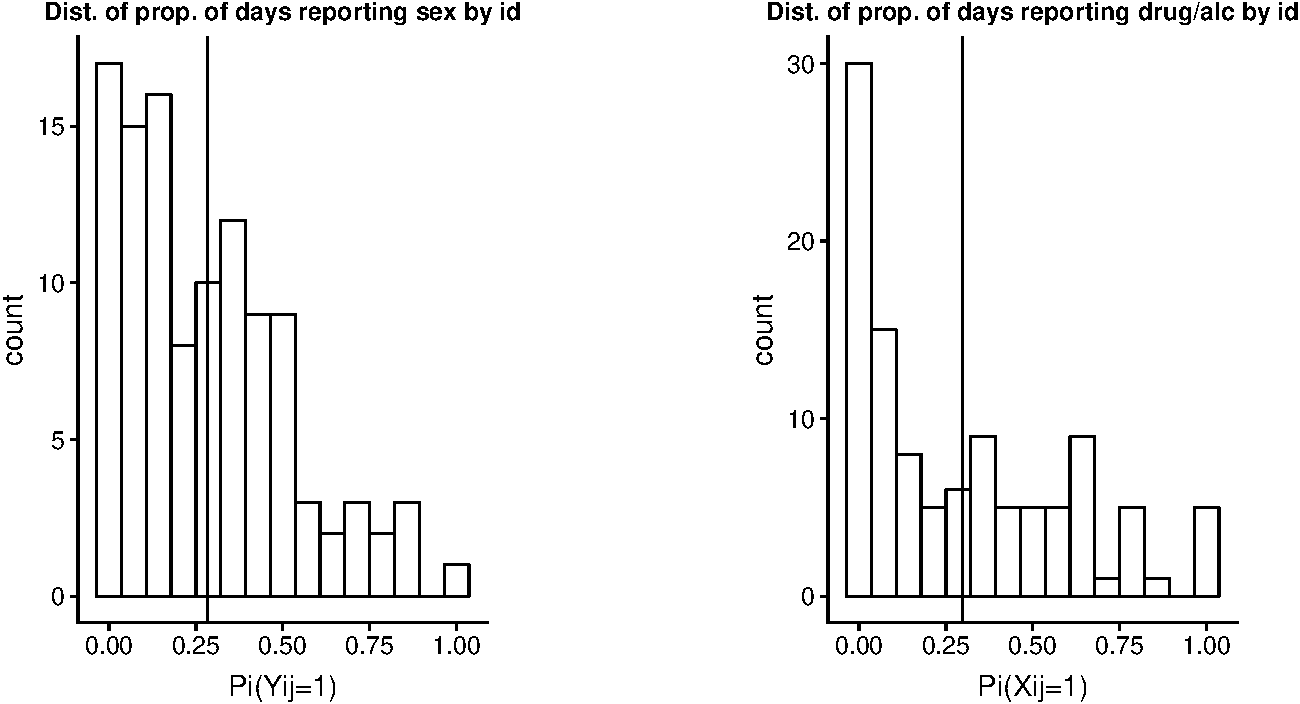
\includegraphics{Chapter5CodePart2_files/figure-beamer/plots-1.pdf}

\end{frame}

\begin{frame}{Comments on data summaries}

\begin{itemize}
\tightlist
\item
  One can see large variation in the proportion of days reported for
  both relevant events (both \(X_{ij},Y_{ij}\)) across individuals.
\item
  Subjects report an average of around 25\% yeses for both variables.
\item
  We will look at ways of modeling this variability below.
\end{itemize}

\end{frame}

\begin{frame}{Transition Models}

-We wish to fit the model:
\[logit[P(Y_{ij}=1 \mid X_{ij}, Y_{i,j-1})] = \beta_0^{TM}+\beta_1^{TM}X_{ij}+\beta_2^{TM} Y_{i,j-1}\]
- We will assume that
\[Y_{ij} \perp (Y_{i1},Y_{i2},\cdots,Y_{i,j-2}) \mid X_{ij},Y_{i,j-1}\]

so, no correlation with past \(Y\)'s given the most recently measured
one.

\begin{itemize}
\tightlist
\item
  First, we need to make a variable of the lagged value of outcome (by 1
  row), ** by id **.
\item
  Note first, that because one of the variables depends on the value the
  next observations, it's blank for the first observation.
\end{itemize}

\end{frame}

\begin{frame}[fragile]{Make lag variable}

\begin{Shaded}
\begin{Highlighting}[]
\NormalTok{knitr}\OperatorTok{::}\KeywordTok{asis_output}\NormalTok{(}\StringTok{"}\CharTok{\textbackslash{}\textbackslash{}}\StringTok{tiny"}\NormalTok{)}
\end{Highlighting}
\end{Shaded}

\tiny

\begin{Shaded}
\begin{Highlighting}[]
\CommentTok{# order by date with eid}
\NormalTok{dat <-}\StringTok{ }\KeywordTok{arrange}\NormalTok{(dat,eid,date)}
\CommentTok{# get new variable which is lagged (by 1) outcome (Y_\{ii,j-1\})}
\NormalTok{dat_new <-}\StringTok{ }\NormalTok{dat }\OperatorTok\StringTok{ }\KeywordTok{group_by}\NormalTok{(eid) }\OperatorTok\StringTok{ }\KeywordTok{mutate}\NormalTok{(}\DataTypeTok{yprev =} \KeywordTok{lag}\NormalTok{(sx24hrs))}
\NormalTok{dat_new[}\DecValTok{22}\OperatorTok{:}\DecValTok{33}\NormalTok{,]}
\end{Highlighting}
\end{Shaded}

\begin{verbatim}
## # A tibble: 12 x 8
## # Groups:   eid [2]
##      eid today     sx24hrs drgalcoh date        year mind       yprev
##    <int> <chr>       <int>    <int> <date>     <dbl> <date>     <int>
##  1     2 3-Jul-98        0        0 1998-07-03  1998 1998-06-04     0
##  2     2 4-Jul-98        0        0 1998-07-04  1998 1998-06-04     0
##  3     2 5-Jul-98        0        0 1998-07-05  1998 1998-06-04     0
##  4     3 4-Jun-98        0        0 1998-06-04  1998 1998-06-04    NA
##  5     3 7-Jun-98        0        0 1998-06-07  1998 1998-06-04     0
##  6     3 8-Jun-98        0        0 1998-06-08  1998 1998-06-04     0
##  7     3 9-Jun-98        0        0 1998-06-09  1998 1998-06-04     0
##  8     3 10-Jun-98       0        0 1998-06-10  1998 1998-06-04     0
##  9     3 11-Jun-98       0        0 1998-06-11  1998 1998-06-04     0
## 10     3 12-Jun-98       0        0 1998-06-12  1998 1998-06-04     0
## 11     3 13-Jun-98       1        1 1998-06-13  1998 1998-06-04     0
## 12     3 14-Jun-98       0        0 1998-06-14  1998 1998-06-04     1
\end{verbatim}

\end{frame}

\begin{frame}{Fit standard logistic regression}

\begin{itemize}
\tightlist
\item
  Given our assumptions of conditional independence above, we have no
  residual correlation of observations on the same subject conditional
  on the past outcome and current drug and alcohol use.
\item
  Thus, we fit the coefficients using standard logistic regression.
\end{itemize}

\end{frame}

\begin{frame}[fragile]{GLM in R}

\begin{Shaded}
\begin{Highlighting}[]
\NormalTok{knitr}\OperatorTok{::}\KeywordTok{asis_output}\NormalTok{(}\StringTok{"}\CharTok{\textbackslash{}\textbackslash{}}\StringTok{tiny"}\NormalTok{)}
\end{Highlighting}
\end{Shaded}

\tiny

\begin{Shaded}
\begin{Highlighting}[]
\NormalTok{glm_tm <-}\StringTok{ }\KeywordTok{glm}\NormalTok{(sx24hrs }\OperatorTok{~}\StringTok{ }\NormalTok{drgalcoh}\OperatorTok{+}\NormalTok{yprev, }\DataTypeTok{data=}\NormalTok{dat_new, }\DataTypeTok{family =}\KeywordTok{binomial}\NormalTok{(),}\DataTypeTok{na.action=}\NormalTok{na.omit)}
\KeywordTok{summary}\NormalTok{(glm_tm)}
\end{Highlighting}
\end{Shaded}

\begin{verbatim}
## 
## Call:
## glm(formula = sx24hrs ~ drgalcoh + yprev, family = binomial(), 
##     data = dat_new, na.action = na.omit)
## 
## Deviance Residuals: 
##     Min       1Q   Median       3Q      Max  
## -1.1673  -0.8823  -0.7142   1.1875   1.7269  
## 
## Coefficients:
##             Estimate Std. Error z value Pr(>|z|)    
## (Intercept) -1.23601    0.07594 -16.276  < 2e-16 ***
## drgalcoh     0.49346    0.12129   4.069 4.73e-05 ***
## yprev        0.71877    0.12079   5.950 2.67e-09 ***
## ---
## Signif. codes:  0 '***' 0.001 '**' 0.01 '*' 0.05 '.' 0.1 ' ' 1
## 
## (Dispersion parameter for binomial family taken to be 1)
## 
##     Null deviance: 1940.6  on 1606  degrees of freedom
## Residual deviance: 1885.2  on 1604  degrees of freedom
##   (301 observations deleted due to missingness)
## AIC: 1891.2
## 
## Number of Fisher Scoring iterations: 4
\end{verbatim}

\end{frame}

\begin{frame}[fragile]{Get associations at right scale}

\begin{itemize}
\tightlist
\item
  See a strong positive relationship of both previous recorded days
  sexual activity as well as current days reporting alcohol/drug use and
  sexual activity.
\item
  We now put into more interpretable odds ratio form. Again, can do this
  several ways, but we'll use the function we've used before. We only
  have binary predictors, so the relevant OR's are just comparing yes
  (1) to no (0) for both.
\end{itemize}

\begin{Shaded}
\begin{Highlighting}[]
\NormalTok{knitr}\OperatorTok{::}\KeywordTok{asis_output}\NormalTok{(}\StringTok{"}\CharTok{\textbackslash{}\textbackslash{}}\StringTok{footnotesize"}\NormalTok{)}
\end{Highlighting}
\end{Shaded}

\footnotesize

\begin{Shaded}
\begin{Highlighting}[]
\KeywordTok{source}\NormalTok{(}\StringTok{"glm_post_estimate.R"}\NormalTok{)}
\NormalTok{comps <-}\StringTok{ }\KeywordTok{rbind}\NormalTok{(}\KeywordTok{c}\NormalTok{(}\DecValTok{0}\NormalTok{,}\DecValTok{1}\NormalTok{,}\DecValTok{0}\NormalTok{),}\KeywordTok{c}\NormalTok{(}\DecValTok{0}\NormalTok{,}\DecValTok{0}\NormalTok{,}\DecValTok{1}\NormalTok{))}
\NormalTok{or_tm <-}\StringTok{ }\KeywordTok{glm.post.estimate}\NormalTok{(glm_tm,comps, }
  \DataTypeTok{labs=}\KeywordTok{c}\NormalTok{(}\StringTok{"drug/alc"}\NormalTok{,}\StringTok{"previousY"}\NormalTok{),}\DataTypeTok{exponentiate =}\NormalTok{ T)            }
\NormalTok{or_tm}
\end{Highlighting}
\end{Shaded}

\begin{verbatim}
##           Ratio.est CI              pvalue 
## drug/alc  "1.638"   "1.291 - 2.078" "0.000"
## previousY "2.052"   "1.619 - 2.600" "0.000"
\end{verbatim}

\end{frame}

\begin{frame}{Interpretation}

\begin{itemize}
\tightlist
\item
  One can see that the estimate odds ratio suggests about a doubling of
  the probability of reporting sexual activity if it was reported the
  previous day (keep drugs and alcohol fixed).

  \begin{itemize}
  \tightlist
  \item
    This obviously suggest a strong correlation of outcomes at least
    over a 1-day interval.
  \end{itemize}
\item
  There is also a strong positive association of drug/alc use in the
  current day versus reported sexual activity.
\end{itemize}

\end{frame}

\begin{frame}{Random (mixed) effects models}

\begin{itemize}
\tightlist
\item
  We will talk extensively about such models in next part of class, but
  for now a brief introduction using the data on teenagers.\\
\item
  This approach implicitly models the correlation by assuming a latent
  variable model that implies correlation of observations made on same
  subject.
\item
  Specifically in this case, the model is:
\end{itemize}

\[logit[P(Y_{ij}=1 \mid X_{ij}, \beta_{0i}] = \beta_0^{RE}+\beta_{0i}+\beta_1^{RE}X_{ij}\]
where it is assumed that the \(\beta_{0i}\) are random, independent
normally distributed variables: \(\beta_{0i} \sim N(0, \tau)\). - This
models assumes that
\[Y_{ij} \perp Y_{ij'}, j' \ne j,  \mid \beta_{0i},X_{ij},\].

\end{frame}

\begin{frame}[fragile]{How to estimate it in R}

\begin{Shaded}
\begin{Highlighting}[]
\NormalTok{knitr}\OperatorTok{::}\KeywordTok{asis_output}\NormalTok{(}\StringTok{"}\CharTok{\textbackslash{}\textbackslash{}}\StringTok{tiny"}\NormalTok{)}
\end{Highlighting}
\end{Shaded}

\tiny

\begin{Shaded}
\begin{Highlighting}[]
\NormalTok{glmer_mod <-}\StringTok{ }\KeywordTok{glmer}\NormalTok{(sx24hrs }\OperatorTok{~}\StringTok{ }\NormalTok{drgalcoh}\OperatorTok{+}\NormalTok{(}\DecValTok{1}\OperatorTok{|}\NormalTok{eid), }\DataTypeTok{data=}\NormalTok{dat_new, }\DataTypeTok{family =}\KeywordTok{binomial}\NormalTok{(),}\DataTypeTok{na.action=}\NormalTok{na.omit)}
\KeywordTok{summary}\NormalTok{(glmer_mod)}
\end{Highlighting}
\end{Shaded}

\begin{verbatim}
## Generalized linear mixed model fit by maximum likelihood (Laplace
##   Approximation) [glmerMod]
##  Family: binomial  ( logit )
## Formula: sx24hrs ~ drgalcoh + (1 | eid)
##    Data: dat_new
## 
##      AIC      BIC   logLik deviance df.resid 
##   1852.1   1868.4   -923.1   1846.1     1705 
## 
## Scaled residuals: 
##     Min      1Q  Median      3Q     Max 
## -1.8638 -0.5799 -0.3905  0.5950  3.6907 
## 
## Random effects:
##  Groups Name        Variance Std.Dev.
##  eid    (Intercept) 1.554    1.247   
## Number of obs: 1708, groups:  eid, 109
## 
## Fixed effects:
##             Estimate Std. Error z value Pr(>|z|)    
## (Intercept)  -1.0815     0.1504  -7.189 6.53e-13 ***
## drgalcoh      0.3908     0.1530   2.554   0.0107 *  
## ---
## Signif. codes:  0 '***' 0.001 '**' 0.01 '*' 0.05 '.' 0.1 ' ' 1
## 
## Correlation of Fixed Effects:
##          (Intr)
## drgalcoh -0.316
\end{verbatim}

\begin{itemize}
\tightlist
\item
  Need slight modification of the glm.post.estimation code to get it to
  work with a lme4 object.
\end{itemize}

\begin{Shaded}
\begin{Highlighting}[]
\NormalTok{knitr}\OperatorTok{::}\KeywordTok{asis_output}\NormalTok{(}\StringTok{"}\CharTok{\textbackslash{}\textbackslash{}}\StringTok{footnotesize"}\NormalTok{)}
\end{Highlighting}
\end{Shaded}

\footnotesize

\begin{Shaded}
\begin{Highlighting}[]
\KeywordTok{source}\NormalTok{(}\StringTok{"glmer_post_estimate.R"}\NormalTok{)}
\NormalTok{comps <-}\StringTok{ }\KeywordTok{c}\NormalTok{(}\DecValTok{0}\NormalTok{,}\DecValTok{1}\NormalTok{)}
\NormalTok{or_re <-}\StringTok{ }\KeywordTok{glmer.post.estimate}\NormalTok{(glmer_mod,comps,}\DataTypeTok{labs=}\KeywordTok{c}\NormalTok{(}\StringTok{"drug/alc"}\NormalTok{),}\DataTypeTok{exponentiate =}\NormalTok{ T)            }
\NormalTok{or_re}
\end{Highlighting}
\end{Shaded}

\begin{verbatim}
##          Ratio.est CI              pvalue 
## drug/alc "1.478"   "1.095 - 1.995" "0.011"
\end{verbatim}

\end{frame}

\begin{frame}[fragile]{get other estimates of unique to the mixed models
( such as \(\tau \equiv SD(\beta_{0i})\))}

\begin{itemize}
\tightlist
\item
  Other information besides ``fixed effect'' coefficients.
\item
  For instance, the standard deviation of the random effects (we just
  have one in this case).\\
\item
  We will spend more time on this later.
\item
  Below is the estimate of \(SD(\beta_{0i})\)
\end{itemize}

\begin{Shaded}
\begin{Highlighting}[]
\KeywordTok{VarCorr}\NormalTok{(glmer_mod)}
\end{Highlighting}
\end{Shaded}

\begin{verbatim}
##  Groups Name        Std.Dev.
##  eid    (Intercept) 1.2465
\end{verbatim}

\end{frame}

\begin{frame}{Generalized Estimating Equation (GEE)}

\begin{itemize}
\tightlist
\item
  Finally, we fit a simple linear model, but use the GEE approach to get
  the inference accounting for the repeated measures.
\item
  As discussed in slides, we can use different working correlation
  matrices to fit the coeffients.
\item
  In this case, we use independence, so the estimates will be the same
  as if done by standard logistic regression.
\item
  However, the robust inference will adjust for the correlation when
  deriving standard errors (SE'S).
\end{itemize}

\end{frame}

\begin{frame}[fragile]{GEE in R}

\begin{Shaded}
\begin{Highlighting}[]
\NormalTok{knitr}\OperatorTok{::}\KeywordTok{asis_output}\NormalTok{(}\StringTok{"}\CharTok{\textbackslash{}\textbackslash{}}\StringTok{tiny"}\NormalTok{)}
\end{Highlighting}
\end{Shaded}

\tiny

\begin{Shaded}
\begin{Highlighting}[]
\NormalTok{gee_fit <-}\StringTok{ }\KeywordTok{gee}\NormalTok{(sx24hrs }\OperatorTok{~}\StringTok{ }\NormalTok{drgalcoh, eid, }\DataTypeTok{data=}\NormalTok{dat_new,}\DataTypeTok{family=}\NormalTok{binomial, }\DataTypeTok{corstr =} \StringTok{"independence"}\NormalTok{)}
\end{Highlighting}
\end{Shaded}

\begin{verbatim}
## Beginning Cgee S-function, @(#) geeformula.q 4.13 98/01/27
\end{verbatim}

\begin{verbatim}
## running glm to get initial regression estimate
\end{verbatim}

\begin{verbatim}
## (Intercept)    drgalcoh 
##   -1.067938    0.553610
\end{verbatim}

\begin{Shaded}
\begin{Highlighting}[]
\CommentTok{# Make easier to read summary}
\NormalTok{ss <-}\StringTok{ }\KeywordTok{data.frame}\NormalTok{(}\KeywordTok{summary}\NormalTok{(gee_fit)}\OperatorTok{$}\NormalTok{coefficients)}
\NormalTok{ss =}\StringTok{ }\KeywordTok{data.frame}\NormalTok{(ss,}\DataTypeTok{pvalue=}\DecValTok{2}\OperatorTok{*}\NormalTok{(}\DecValTok{1}\OperatorTok{-}\KeywordTok{pnorm}\NormalTok{(}\KeywordTok{abs}\NormalTok{(ss[,}\DecValTok{5}\NormalTok{]))))}
\KeywordTok{round}\NormalTok{(ss,}\DecValTok{4}\NormalTok{)}
\end{Highlighting}
\end{Shaded}

\begin{verbatim}
##             Estimate Naive.S.E.  Naive.z Robust.S.E. Robust.z pvalue
## (Intercept)  -1.0679     0.0648 -16.4707      0.1100  -9.7085 0.0000
## drgalcoh      0.5536     0.1164   4.7543      0.1802   3.0714 0.0021
\end{verbatim}

We need slightly altered functions to get post-hoc estimates of linear
combination of coefficients.

\begin{Shaded}
\begin{Highlighting}[]
\NormalTok{knitr}\OperatorTok{::}\KeywordTok{asis_output}\NormalTok{(}\StringTok{"}\CharTok{\textbackslash{}\textbackslash{}}\StringTok{tiny"}\NormalTok{)}
\end{Highlighting}
\end{Shaded}

\tiny

\begin{Shaded}
\begin{Highlighting}[]
\KeywordTok{source}\NormalTok{(}\StringTok{"gee_post_estimate.R"}\NormalTok{)}
\NormalTok{comps <-}\StringTok{ }\KeywordTok{c}\NormalTok{(}\DecValTok{0}\NormalTok{,}\DecValTok{1}\NormalTok{)}
\NormalTok{or_gee <-}\StringTok{ }\KeywordTok{gee.post.estimate}\NormalTok{(gee_fit,comps,}\DataTypeTok{labs=}\KeywordTok{c}\NormalTok{(}\StringTok{"drug/alc"}\NormalTok{),}\DataTypeTok{exponentiate =}\NormalTok{ T)            }
\NormalTok{or_gee}
\end{Highlighting}
\end{Shaded}

\begin{verbatim}
##          Ratio.est CI              pvalue 
## drug/alc "1.740"   "1.222 - 2.477" "0.002"
\end{verbatim}

\end{frame}

\begin{frame}{Comparing GEE/RE model}

\begin{itemize}
\item
  One can see that, though both the GEE approach and the random effects
  model account for correlation when deriving their inference, they give
  quite different estimates of the the OR (1.478 versus 1.740).
\item
  Why??
\end{itemize}

\end{frame}

\begin{frame}{Different correlation model for GEE}

\begin{itemize}
\item
  Now we do a GEE model again, but using a different working correlation
  model (exchangeable in this case).
\item
  This one assumes that all observations on the same individual are
  equally correlated.
\item
  It just involves one small change in the gee function.
\end{itemize}

\end{frame}

\begin{frame}[fragile]{Re-fit with exchangeable working correlation}

\begin{Shaded}
\begin{Highlighting}[]
\NormalTok{knitr}\OperatorTok{::}\KeywordTok{asis_output}\NormalTok{(}\StringTok{"}\CharTok{\textbackslash{}\textbackslash{}}\StringTok{tiny"}\NormalTok{)}
\end{Highlighting}
\end{Shaded}

\tiny

\begin{Shaded}
\begin{Highlighting}[]
\NormalTok{gee_fit <-}\StringTok{ }\KeywordTok{gee}\NormalTok{(sx24hrs }\OperatorTok{~}\StringTok{ }\NormalTok{drgalcoh, eid, }\DataTypeTok{data=}\NormalTok{dat_new,}\DataTypeTok{family=}\NormalTok{binomial, }\DataTypeTok{corstr =} \StringTok{"exchangeable"}\NormalTok{)}
\end{Highlighting}
\end{Shaded}

\begin{verbatim}
## Beginning Cgee S-function, @(#) geeformula.q 4.13 98/01/27
\end{verbatim}

\begin{verbatim}
## running glm to get initial regression estimate
\end{verbatim}

\begin{verbatim}
## (Intercept)    drgalcoh 
##   -1.067938    0.553610
\end{verbatim}

\begin{Shaded}
\begin{Highlighting}[]
\CommentTok{# Make easier to read summary}
\NormalTok{ss <-}\StringTok{ }\KeywordTok{data.frame}\NormalTok{(}\KeywordTok{summary}\NormalTok{(gee_fit)}\OperatorTok{$}\NormalTok{coefficients)}
\NormalTok{ss =}\StringTok{ }\KeywordTok{data.frame}\NormalTok{(ss,}\DataTypeTok{pvalue=}\DecValTok{2}\OperatorTok{*}\NormalTok{(}\DecValTok{1}\OperatorTok{-}\KeywordTok{pnorm}\NormalTok{(}\KeywordTok{abs}\NormalTok{(ss[,}\DecValTok{5}\NormalTok{]))))}
\KeywordTok{round}\NormalTok{(ss,}\DecValTok{4}\NormalTok{)}
\end{Highlighting}
\end{Shaded}

\begin{verbatim}
##             Estimate Naive.S.E. Naive.z Robust.S.E. Robust.z pvalue
## (Intercept)  -0.8751     0.1071 -8.1700      0.1163  -7.5274 0.0000
## drgalcoh      0.3321     0.1188  2.7941      0.1371   2.4219 0.0154
\end{verbatim}

\begin{Shaded}
\begin{Highlighting}[]
\NormalTok{or_gee_exch <-}\StringTok{ }\KeywordTok{gee.post.estimate}\NormalTok{(gee_fit,comps,}\DataTypeTok{labs=}\KeywordTok{c}\NormalTok{(}\StringTok{"drug/alc"}\NormalTok{),}\DataTypeTok{exponentiate =}\NormalTok{ T)            }
\NormalTok{or_gee_exch}
\end{Highlighting}
\end{Shaded}

\begin{verbatim}
##          Ratio.est CI              pvalue 
## drug/alc "1.394"   "1.065 - 1.824" "0.015"
\end{verbatim}

\end{frame}

\begin{frame}{Comparing independence and exchangeable working
correlation}

\begin{itemize}
\item
  As one can see, there is also a big difference in the estimate of the
  odds ratio of drug/alcohol for two different runs of the GEE approach,
  but with different working correlation models.
\item
  Why?
\end{itemize}

\end{frame}

\end{document}
